% !TeX root = ../main.tex
\section{Results}\label{sec:results}

\subsection{Sentinel-1 signatures of historical stand disturbances}


Historical BALSA stand disturbances exhibited repeatable negative Sentinel-1 responses (Fig.~\ref{fig:s1_population_signatures}). The distributional analysis used all valid polygon-month observations from the 3,498 validated polygons; 1,018 events in 462 polygons had the paired temporal support required for the event-level summaries. Across all valid polygon-month medians, the 5th--95th percentile ranges were $-9.3$ to $-5.0$~dB for VV and $-15.7$ to $-11.5$~dB for VH. Median VV changed from $-6.0$~dB before disturbance to $-7.5$~dB during months 0 to $+2$, while VH changed from $-12.5$ to $-14.0$~dB. The pre- and post-event distributions nevertheless remained broadly overlapping, so neither polarization defined a stable national absolute threshold (Fig.~\ref{fig:s1_population_signatures}a).

\begin{figure}[pos=!htbp]
    \centering
    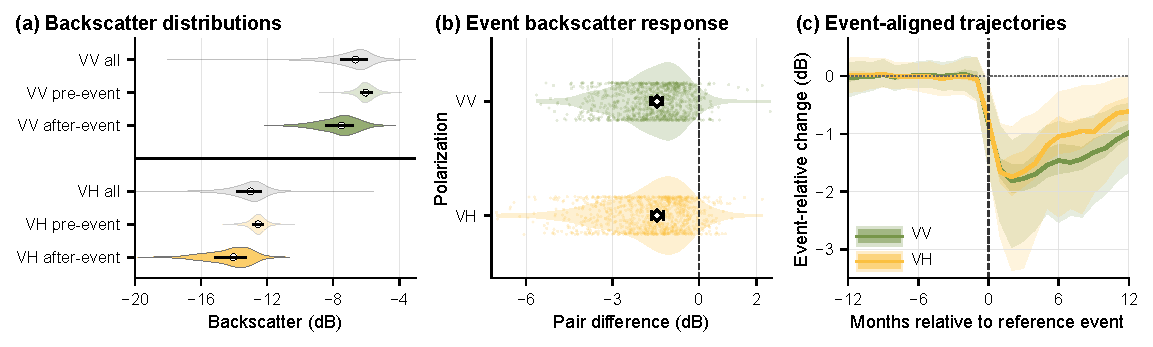
\includegraphics[width=1.0\textwidth]{figures/fig05_population_s1_signatures.pdf}
    \caption{Sentinel-1 signatures of historical balsa stand disturbances. (a) VV and VH distributions across all valid observations from the 3,498 validated BALSA polygons and during the pre-event ($-12$ to $-3$ months) and post-event (0 to $+2$ months) periods. (b) Paired post-minus-pre-event differences for 1,018 dated events; diamonds show medians and bars show 95\% complete-spatial-block bootstrap intervals. (c) Event-aligned changes relative to the pre-event background. Dark and light ribbons show interquartile ranges and pointwise 95\% block-bootstrap intervals, respectively.}
    \label{fig:s1_population_signatures}
\end{figure}
\FloatBarrier

Within-event contrasts were more consistent than the absolute values. Median post-minus-pre-event backscatter was $-1.5$~dB for VV (95\% complete-spatial-block bootstrap interval, $-1.7$ to $-1.3$~dB) and $-1.5$~dB for VH ($-1.6$ to $-1.2$~dB); 96.4\% and 94.1\% of the respective changes were negative (Fig.~\ref{fig:s1_population_signatures}b). The median deviations reached approximately $-1.8$~dB by month $+2$ and remained negative at month $+12$ ($-1.0$~dB for VV and $-0.6$~dB for VH). Pointwise 95\% spatial-block bootstrap intervals remained below zero from month 0 through month $+12$ for both polarizations (Fig.~\ref{fig:s1_population_signatures}c).


The representative polygon showed the same stand-scale response
(Fig.~\ref{fig:timeseries_signature}). Polygon-level median and mean
trajectories preserved the major disturbance valleys, and the March 2024
reference event coincided with coherent VV/VH declines and an optical
transition from dense canopy to exposed ground. Similar absolute
backscatter levels occurred during recovery and subsequent disturbance,
further supporting characterization relative to each stand's recent state.


\begin{figure}[pos=!htbp]
    \centering
    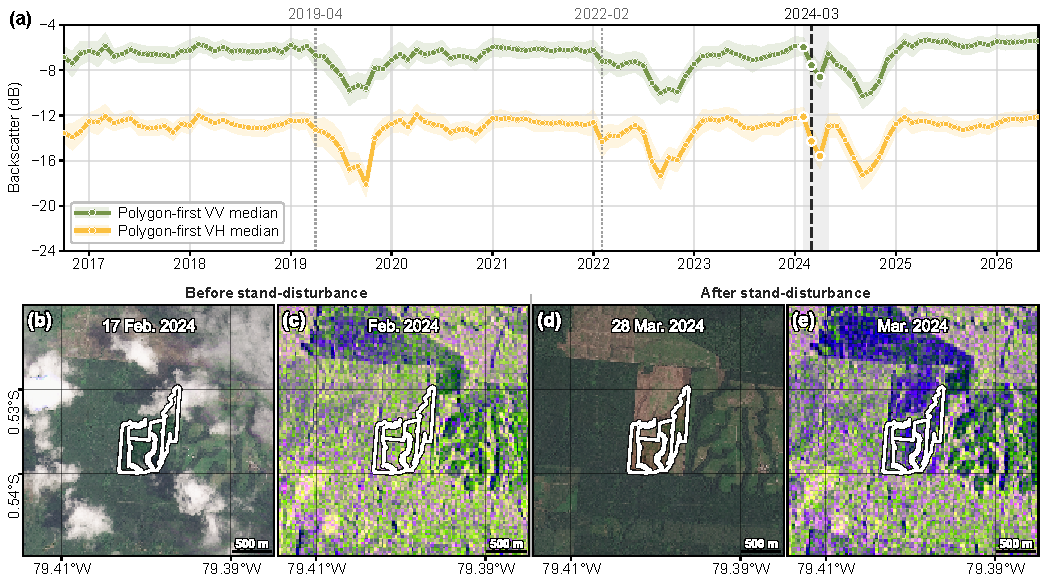
\includegraphics[width=\linewidth]{figures/fig06_representative_timeseries.pdf}
    \caption{Sentinel-1 and optical observations of a representative balsa plantation. (a) Monthly Polygon-first VV and VH median backscatter from October 2016 to June 2026. Shading denotes the within-polygon pixel interquartile range for each polarization, and vertical lines mark independently interpreted reference-event months. (b,c) PlanetScope and Sentinel-1 observations before the March 2024 event. (d,e) Corresponding observations after the event. Sentinel-1 false-colour composites use R = VV, G = VH, and B = VV$-$VH; scale bars represent 500~m.}
    \label{fig:timeseries_signature}
\end{figure}
\FloatBarrier



\subsection{Stand representation and configuration sensitivity}
\label{sec:representation_configuration}




We next evaluated the sensitivity of disturbance detection to stand representation, temporal window geometry, and polarization strategy.


\begin{figure*}[pos=!htbp]
    \centering
    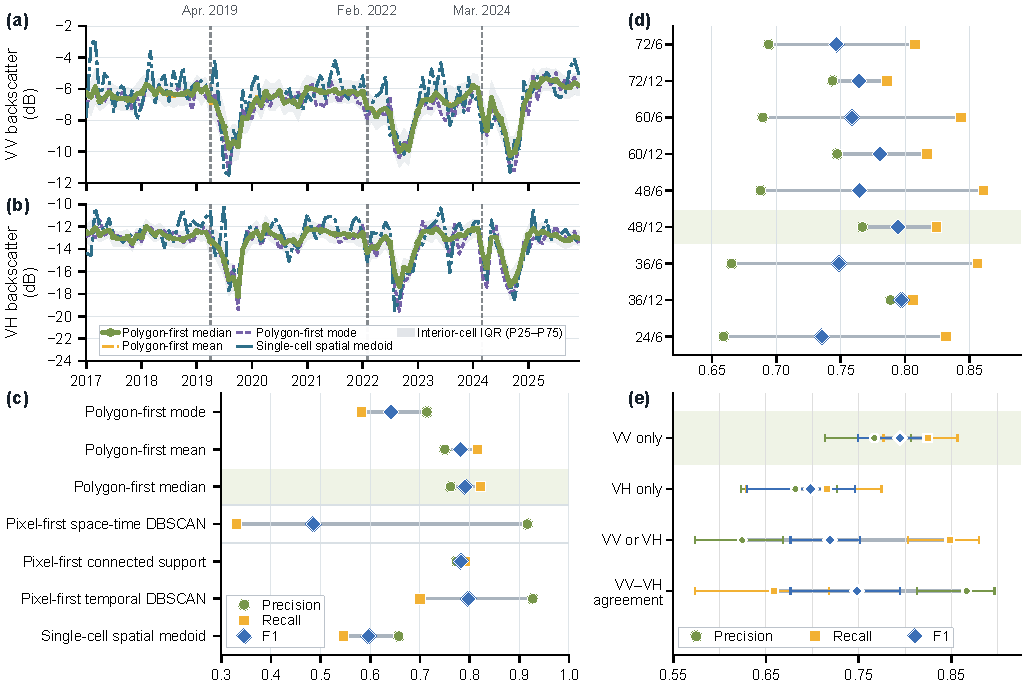
\includegraphics[width=\linewidth]{figures/fig07_representation_configuration.pdf}
    \caption{Sensitivity of Windowed CUSUM to stand representation, temporal window geometry, and polarization strategy. (a,b) Illustrative VV and VH stand trajectories with cell-level interquartile ranges and reference disturbances. (c--e) Event-level precision, recall, and F1 across stand representations, window configurations, and polarization strategies, respectively. Whiskers denote 95\% spatial-block bootstrap confidence intervals, and pale-green highlighting indicates the retained configurations.}
    \label{fig:stand_representation_sensitivity}
\end{figure*}

Under the fixed 48/12 configuration, the Polygon-first median achieved precision 0.762, recall 0.823, and F1 0.791 (Fig.~\ref{fig:stand_representation_sensitivity}~(c)). Alternative representations produced no detectable F1 improvement; even temporal DBSCAN, which had the highest alternative point estimate (F1 = 0.798), differed from the median by only $+0.007$ (95\% CI: $-0.032$ to 0.042). The Polygon-first median was therefore retained because it preserved high recall without requiring pixel-support or clustering parameters.


Across the evaluated window geometries, 12-month displacements generally favored F1 over six-month displacements (Fig.~\ref{fig:stand_representation_sensitivity}~(d)). The highest fixed F1 was 0.797 for 36/12, only 0.003 above the prospectively locked 48/12 configuration (95\% CI: $-0.013$ to 0.019). Although 36/12 was selected in all five outer folds, nested spatial out-of-fold F1 was 0.796. The prespecified 48/12 geometry was therefore retained.



VV-only detection produced the highest F1 (0.795; precision 0.767, recall 0.824; Fig.~\ref{fig:stand_representation_sensitivity}~(e)). Either-polarization fusion increased recall but reduced precision, whereas VV--VH agreement produced the opposite trade-off; neither improved F1. VV was therefore retained as the operational input.



\subsection{Component attribution of the proposed Windowed CUSUM}
\label{sec:representation_component_ablation}


Progressive component analysis identified local-reference windowing and central-interval admission as the two largest incremental contributors (Table~\ref{tab:component_ablation}). Windowing primarily increased recall ($\Delta F1=+0.137$, 95\% CI: 0.075--0.198), whereas the central interval recovered precision ($\Delta F1=+0.127$, 0.103--0.146). Permutation screening provided a further F1 gain of 0.036 (0.022--0.049), while the negative-shift constraint had negligible discriminative effect.


\begin{table*}[pos=!htbp]
    \centering
    \small
    \caption{Progressive component analysis under the fixed 48/12 configuration. $\Delta F1$ compares adjacent configurations; intervals are paired spatial-block bootstrap 95\% CIs.}
    \label{tab:component_ablation}
    \begin{tabular}{lccccc}
        \toprule
        Cumulative configuration
        & Detections
        & Precision
        & Recall
        & F1
        & Incremental $\Delta F1$ [95\% CI] \\
        \midrule

        Global CUSUM
        & 447
        & 0.852
        & 0.349
        & 0.495
        & -- \\

        + Local-reference windows
        & 1,948
        & 0.493
        & 0.878
        & 0.631
        & $+0.137$ [0.075, 0.198] \\

        + Central decision interval
        & 1,362
        & 0.684
        & 0.852
        & 0.758
        & $+0.127$ [0.103, 0.146] \\

        + Negative-shift constraint
        & 1,350
        & 0.687
        & 0.848
        & 0.759
        & $+0.000$ [$-0.003$, 0.003] \\

        + Permutation-based screening
        & 1,175
        & 0.767
        & 0.824
        & \textbf{0.795}
        & $+0.036$ [0.022, 0.049] \\

        \bottomrule
    \end{tabular}
\end{table*}


Additional controlled removal produced the same ordering. The full-minus-removedF1 contrast was largest for local-reference windowing ($+0.327$, 95\% CI: 0.280--0.370), compared with $+0.038$ for the central interval and $+0.036$ for permutation screening; removal of the negative-shift constraint had negligible effect. Both analyses therefore identified local-reference windowing as the principal source of recurrent-event sensitivity.


\FloatBarrier


\subsection{Benchmark comparison and statistical robustness}
\label{sec:benchmark_null_sensitivity}

For external benchmarking, Windowed CUSUM achieved precision 0.787, recall 0.805, F1 0.796, and temporal MAE 0.778 months (Table~\ref{tab:benchmark_comparison}). The strongest alternative, decrease-filtered ReCuSum, matched its precision (0.787) but had lower recall (0.591; F1 = 0.675), yielding a paired F1 advantage of $+0.122$ (95\% CI: 0.094--0.149). The benchmark advantage therefore arose primarily from recurrent-event recall.


\begin{table}[pos=!htbp]
    \centering
    \small
    \caption{Nested five-fold spatial out-of-fold comparison of disturbance detectors using common Polygon-first median trajectories and a $\pm2$-month event-matching tolerance. Temporal MAE was calculated for matched events only.}
    \label{tab:benchmark_comparison}

    \begin{tabular}{lcccc}
        \toprule
        Method
        & Precision
        & Recall
        & F1
        & MAE (months) \\
        \midrule

        \textbf{Windowed CUSUM}
        & 0.787
        & 0.805
        & \textbf{0.796}
        & 0.778 \\

        ReCuSum, decrease-filtered
        & 0.787
        & 0.591
        & 0.675
        & 0.752 \\

        f-pol BOCD, decrease-filtered
        & 0.740
        & 0.343
        & 0.469
        & 0.747 \\

        ReCuSum, raw
        & 0.419
        & 0.513
        & 0.461
        & 0.743 \\

        Maximum monthly decline
        & 0.335
        & 0.572
        & 0.422
        & 0.755 \\

        Classical lower CUSUM
        & 0.171
        & 0.290
        & 0.215
        & 1.498 \\

        BFAST-style, decrease-filtered
        & 0.679
        & 0.101
        & 0.175
        & 0.673 \\

        \bottomrule
    \end{tabular}
\end{table}



Separately, temporal-null formulation altered the precision--recall operating point (Table~\ref{tab:temporal_null_sensitivity}). Finite-sample correction of the independent-value permutation changed F1 only from 0.791 to 0.795. In contrast, preserving temporal dependence made screening more selective. A three-month calendar-block permutation increased precision from 0.767 to 0.828 but reduced recall from 0.824 to 0.676 ($\Delta F1=-0.050$, 95\% CI: $-0.084$ to $-0.028$), with stronger dependence-preserving formulations producing still lower recall. Monte Carlo seed variation was negligible relative to differences among null formulations. Under the common threshold, the finite-sample independent-value permutation retained the highest F1.


\begin{table*}[pos=!htbp]
    \centering
    \small
    \caption{Sensitivity of Windowed CUSUM to alternative temporal-null formulations for permutation-based screening under the fixed 48-month window, 12-month displacement, and $\pm2$-month event-matching tolerance. MBB denotes residual moving-block bootstrap and maxT denotes a track-wise maximum-statistic block null.}
    \label{tab:temporal_null_sensitivity}

    \begin{tabular}{llcccc}
        \toprule
        Temporal-null formulation
        & Block length
        & Detections
        & Precision
        & Recall
        & F1 \\
        \midrule

        Archived empirical-rank IID implementation
        & --
        & 1,180
        & 0.762
        & 0.823
        & 0.791 \\

        \textbf{Finite-sample-corrected IID permutation}
        & --
        & 1,175
        & 0.767
        & 0.824
        & \textbf{0.795} \\

        Calendar-block permutation
        & 3 months
        & 892
        & 0.828
        & 0.676
        & 0.745 \\

        Calendar-block permutation
        & 6 months
        & 410
        & 0.902
        & 0.339
        & 0.492 \\

        Calendar-block permutation
        & 12 months
        & 0
        & --
        & 0.000
        & 0.000 \\

        Residual MBB
        & 3 months
        & 927
        & 0.790
        & 0.670
        & 0.725 \\

        Residual MBB
        & 6 months
        & 830
        & 0.772
        & 0.586
        & 0.667 \\

        Residual MBB
        & 12 months
        & 897
        & 0.761
        & 0.625
        & 0.686 \\

        Track-wise maxT block null
        & 3 months
        & 272
        & 0.915
        & 0.228
        & 0.365 \\

        \bottomrule
    \end{tabular}
\end{table*}

Dependence-aware temporal nulls produced a clearer precision--recall trade-off. A three-month calendar-block permutation increased precision from 0.767 to 0.828 but reduced recall from 0.824 to 0.676, lowering F1 to 0.745 ($\Delta F1=-0.050$, 95\% CI: $-0.084$ to $-0.028$). Increasing the block length made candidate admission progressively more conservative; recall declined to 0.339 with six-month blocks, while the 12-month formulation admitted no events. The track-wise maximum-statistic block null showed a similar pattern, achieving precision of 0.915 but recall of only 0.228 (F1 = 0.365).

Residual moving-block-bootstrap nulls produced intermediate results, with F1 ranging from 0.667 to 0.725 across block lengths of 3--12 months. Monte Carlo variation across random seeds was negligible relative to the differences among temporal-null formulations. Under the common $p_{\mathrm{perm}}\leq0.025$ threshold, the finite-sample-corrected IID permutation produced the highest overall F1, whereas increasingly dependence-preserving nulls systematically shifted the detector toward higher selectivity and lower recall.

\subsection{Temporal truncation and prospective performance}
Temporal truncation showed that detection sensitivity increased substantially as post-disturbance observations accumulated. Among the 1,065 reference events evaluable at every horizon, recall increased from 0.202 using observations available only through the reference month to 0.613 after three months, 0.790 after six months, and 0.849 after 12 months. Event dates were comparatively stable once detections had been established: of the 841 reference events detected by the six-month horizon, 814 (96.8\%) were assigned a disturbance month within two months of their corresponding 12-month estimate.

When the locked Windowed CUSUM configuration was subsequently replayed using observations through June 2026, it produced 139 provisional disturbance candidates. Manual review was conducted for 95 sampled candidate polygons. After accounting for the tier-specific sampling fractions, 57.5\% of candidates were estimated to represent confirmed disturbances (95\% spatial-block bootstrap CI: 0.287--0.812), increasing to 64.0\% (95\% CI: 0.393--0.846) when probable disturbances were also included.
\FloatBarrier

\subsection{Recurrent disturbance intervals and plantation rotation dynamics}
\label{sec:rotation_dynamics}

Applying the VV-only Windowed CUSUM to all validated BALSA polygons identified 6,658 qualified disturbance events during 2017--2025. Among these, 2,194 polygons contained at least two events and provided 3,509 intervals between consecutive disturbances. As shown in Fig.~\ref{fig:national_recurrence_patterns}~(d), the median observed inter-disturbance interval was 36 months (IQR: 22--46 months; 95\% spatial-block bootstrap CI: 35--38 months). More than half of all intervals (53.0\%) occurred between 24 and 47 months, and 74.3\% were at least 24 months. Short intervals were also present, with 20.4\% shorter than 12 months, indicating that not every pair of successive detections can be interpreted as a complete plantation rotation.

\begin{figure*}[pos=!htbp]
    \centering
    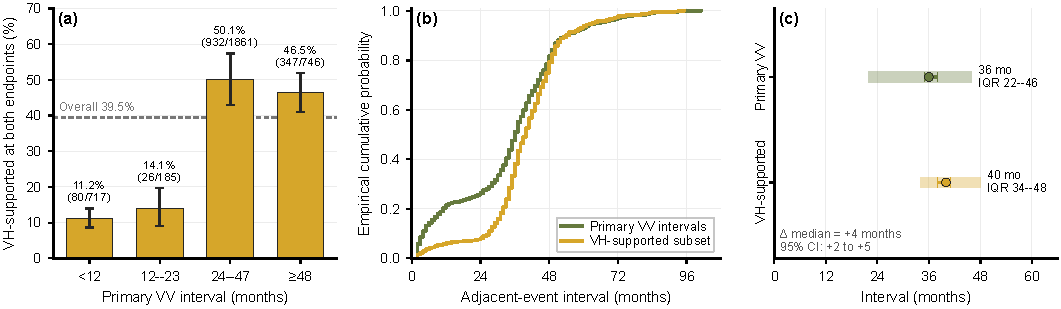
\includegraphics[width=\linewidth]{figures/fig08_polarization_intervals.pdf}
    \caption{Cross-polarization sensitivity of observed inter-disturbance intervals. (a) Fraction of VV-defined intervals for which both bounding disturbance events had corresponding VH detections within $\pm2$ months. (b) Empirical cumulative distributions of all VV intervals ($n=3{,}509$) and the cross-polarization-consistent subset ($n=1{,}385$). (c) Median and interquartile interval estimates with 95\% spatial-block bootstrap confidence intervals.}
    \label{fig:polarization_interval_sensitivity}
\end{figure*}

To assess whether the approximately three-year recurrence was specific to the VV-derived disturbance sequence, we performed a cross-polarization robustness analysis using VH. Cross-polarization filtering retained 1,385 intervals from 1,081 polygons (39.5\% of VV intervals). Their median was 40 months (IQR: 34--48; 95\% CI: 38--41), four months longer than the primary VV estimate (paired 95\% CI: $+2$ to $+5$ months), indicating that the dominant approximately three-year recurrence persisted with VH support. VH support was substantially less frequent for intervals shorter than
24 months than for longer intervals, indicating preferential retention of longer recurrence periods rather than an unbiased refinement of the VV estimate.



These intervals represent recurrent stand turnover observed within the Sentinel-1 record. Notably, individual negative disturbance events could not always be independently attributed to clear-cut harvesting. The 36-month median is therefore interpreted as a rotation-relevant recurrence timescale of observed plantation turnover.

Application of the VV-only Windowed CUSUM to 3,498 validated BALSA polygons identified 6,658 disturbance events during 2017--2025 (Fig.~\ref{fig:national_recurrence_patterns}). Event recurrence showed marked spatial heterogeneity (Fig.~\ref{fig:national_recurrence_patterns}~(a)), while annual detections ranged from 308 in 2023 to 1,026 in 2022 (Fig.~\ref{fig:national_recurrence_patterns}~(b)). The 2023 minimum coincided with the post-boom contraction that followed the 2019--2021 balsa fever, when exceptional wind-sector demand rapidly depleted mature plantation stocks and Ecuadorian balsa exports subsequently declined sharply~\citep{Sanchez2023BalsaExports,EIA2024IllWind}. As shown in Fig.~\ref{fig:national_recurrence_patterns}~(c), 82.9\% of the inventory contained one to three detected events and 349 plots contained none. The 2,194 stands with at least two events provided 3,509 consecutive inter-disturbance intervals, with a median of 36 months (IQR: 22--46 months; 95\% spatial-block bootstrap CI: 35--38 months; Fig.~\ref{fig:national_recurrence_patterns}d).

\FloatBarrier
